\documentclass[11pt]{scrartcl}
\usepackage{dominatrix}
\usepackage{colortbl}
\usepackage{pgfplots}
\pgfplotsset{compat=1.9}
\renewcommand\thesubsection{\alph{subsection}}
\definecolor{light-gray}{gray}{0.75}

\newcommand{\n}[1]{\ensuremath{\text{#1}}}

\title{Problem Set 2: Analytical}
\subject{Natural Language Processing}
\author{Linan Qiu (lq2137)}
\begin{document}
\maketitle

\section{PCFG Transformation to Chomsky Normal Form}

\subsection{Transformation Algorithm}

The following recursive algorithm reduces rules with more than 2 non-terminals to rules with 2 non-terminals (Chomsky Normal Form)

\begin{itemize}
\item Let rule $\n{A} \rightarrow \n{B}_1 \n{B}_2 \n{B}_3 ... \n{B}_n$
\begin{itemize}
\item If $n = 2$ (e.g. $\n{A} \rightarrow \n{B}_1 \n{B}_2$), leave it as it is
\item If $n > 2$,
\begin{itemize}
\item Delete rule $\n{A} \rightarrow \n{B}_1 ... \n{B}_n$
\item Create new rule $A \rightarrow \n{B}_1 \n{C}$ where $\n{C}$ is a newly created non-terminal. Set P($\n{A} \rightarrow \n{B}_1 \n{C}) = P(\n{A} \rightarrow \n{B}_1 \n{B}_2 \n{B}_3 ... \n{B}_n)$
\item Create new rule $\n{C} \rightarrow \n{B}_2 ... \n{B}_n$. Set $P(\n{C} \rightarrow \n{B}_2 ... \n{B}_n) = 1$ since we are sure that this newly created rule goes only to the subsequence originally on the right
\item Apply this algorithm on rule $\n{C} \rightarrow \n{B}_2 ... \n{B}_n$ until $n=2$
\end{itemize}
\end{itemize}
\item Set $P(A \rightarrow \n{B}_1 \n{B}_2 \n{B}_3 ... \n{B}_n) = P(A \rightarrow \n{B}_1 \n{C}_1) P(\n{C}_1 \rightarrow \n{B}_2 \n{C}_2) ... P(\n{C}_{n-2} \rightarrow \n{B}_{n-1} \n{B}_n)$
\end{itemize}

\subsection{Transforming $G'$}

There are 3 rules we need to expand

\begin{itemize}
\item $\n{S} \rightarrow \n{NP NP VP}$
\begin{itemize}
\item $\n{S} \rightarrow \n{NP NP-VP}$, $P=0.3$
\item $\n{NP-VP} \rightarrow \n{NP VP}$, $P=1$
\end{itemize}

\item $\n{VP} \rightarrow \n{Vt NP PP}$
\begin{itemize}
\item $\n{VP} \rightarrow \n{Vt NP-PP}$, $P=0.2$
\item $\n{NP-PP} \rightarrow \n{NP PP}$, $P=1$
\end{itemize}

\item $\n{NP} \rightarrow \n{DT NN NN}$
\begin{itemize}
\item $\n{NP} \rightarrow \n{DT NN-NN}$, $P=0.3$
\item $\n{NN-NN} \rightarrow \n{NN NN}$, $P=1$
\end{itemize}
\end{itemize}

Hence the resulting non-terminal rules for grammar $G$ is

\begin{table}[H]
\centering
\begin{tabular}{r c l l c}
\toprule
\multicolumn{4}{c}{Rule} & Probability \\
\midrule
S & $\rightarrow$ & NP & VP & 0.7 \\
S & $\rightarrow$ & NP & NP-VP & 0.3 \\ 
NP-VP & $\rightarrow$ & NP & VP & 1 \\
VP & $\rightarrow$ & Vt & NP & 0.8 \\
VP & $\rightarrow$ & Vt & NP-PP & 0.2 \\
NP-PP & $\rightarrow$ & NP & PP & 1 \\
NP & $\rightarrow$ & DT & NN-NN & 0.3 \\
NN-NN & $\rightarrow$ & NN & NN & 1 \\
NP & $\rightarrow$ & NP & PP & 0.7 \\ 
PP & $\rightarrow$ & IN & NP & 1.0 \\
\bottomrule
\end{tabular}
\caption{Non-Terminal Rules}
\label{table:nonterminal_rules}
\end{table}

The terminal rules are unchanged.

\section{Treebank}

\subsection{PCFG}

\begin{table}[H]
\centering
\begin{tabular}{r c l l c}
\toprule
\multicolumn{4}{c}{Rule} & Probability \\
\midrule
S & $\rightarrow$ & NP & VP & 1 \\[2ex]
SBAR & $\rightarrow$ & COMP & S & 1 \\[2ex]
VP & $\rightarrow$ & V1 & SBAR & $\frac{1}{3}$ \\[2ex]
VP & $\rightarrow$ & V2 &  & $\frac{1}{3}$ \\[2ex]
VP & $\rightarrow$ & VP & ADVP & $\frac{1}{3}$ \\[2ex]
\midrule
V1 & $\rightarrow$ & said &  & $\frac{1}{3}$ \\[2ex]
V1 & $\rightarrow$ & declared &  & $\frac{1}{3}$ \\[2ex]
V1 & $\rightarrow$ & pronounced &  & $\frac{1}{3}$ \\[2ex]
V2 & $\rightarrow$ & snored &  & $\frac{1}{3}$ \\[2ex]
V2 & $\rightarrow$ & ran &  & $\frac{1}{3}$ \\[2ex]
V2 & $\rightarrow$ & swarm &  & $\frac{1}{3}$ \\[2ex]
ADVP & $\rightarrow$ & loudly &  & $\frac{1}{3}$ \\[2ex]
ADVP & $\rightarrow$ & quickly &  & $\frac{1}{3}$ \\[2ex]
ADVP & $\rightarrow$ & elegantly &  & $\frac{1}{3}$ \\[2ex]
COMP & $\rightarrow$ & that &  & 1 \\[2ex]
NP & $\rightarrow$ & John &  & $\frac{1}{6}$ \\[2ex]
NP & $\rightarrow$ & Sally &  & $\frac{1}{3}$ \\[2ex]
NP & $\rightarrow$ & Bill &  & $\frac{1}{6}$ \\[2ex]
NP & $\rightarrow$ & Fred &  & $\frac{1}{6}$ \\[2ex]
NP & $\rightarrow$ & Jeff &  & $\frac{1}{6}$ \\[2ex]
\bottomrule
\end{tabular}
\caption{PCFG for Treebank}
\label{table:pcfg_treebank}
\end{table}

\subsection{Parse Trees}

\begin{figure}[H]
\centering
\scalebox{0.6}{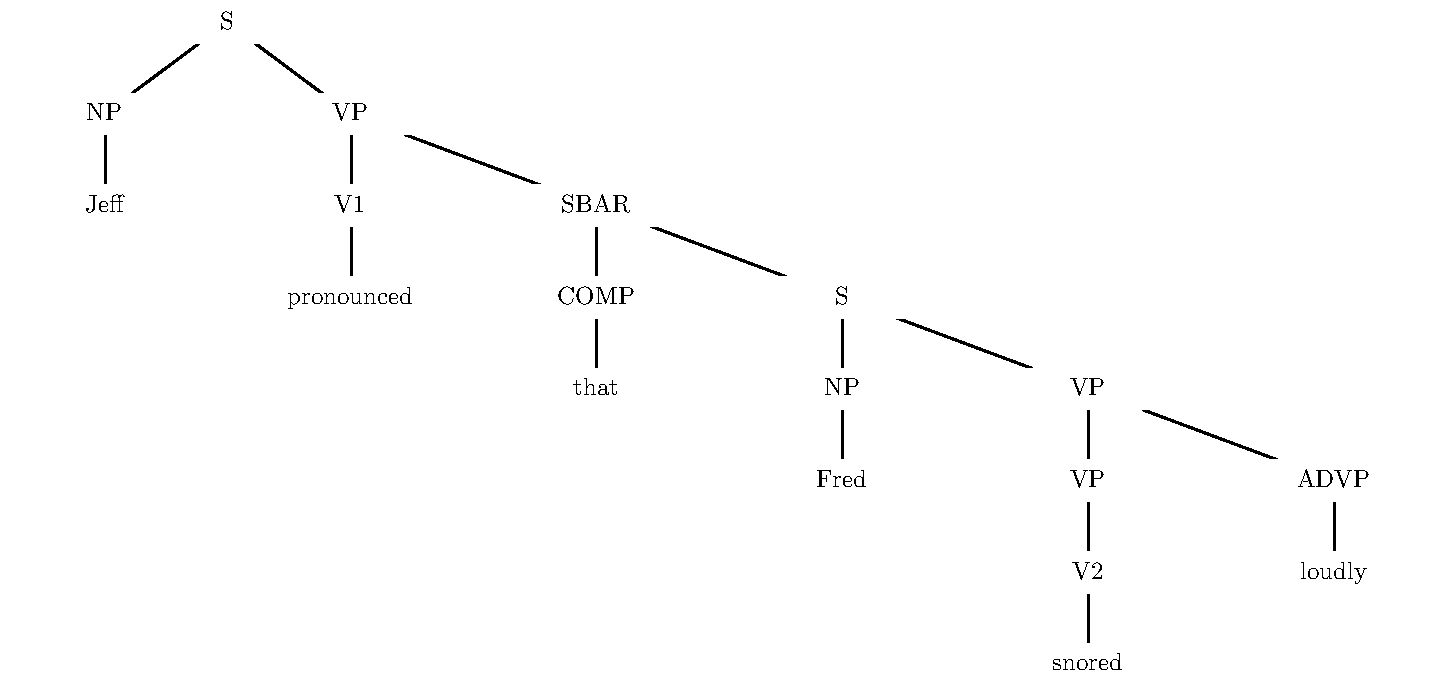
\includegraphics[]{h2-2-parsetree1.pdf}}
\caption{Parse Tree 1: Jeff accusing Fred of snoring loudly.}
\label{fig:parse_tree_1}
\end{figure}

\begin{align*}
P_{\tau_1} &= [ P(\n{S} \rightarrow \n{NP VP}) * P(\n{VP} \rightarrow \n{V1 SBAR}) * P(\n{SBAR} \rightarrow \n{COMP S}) * P(\n{S} \rightarrow \n{NP VP}) \\
&* P(\n{VP} \rightarrow \n{VP ADVP}) * P(\n{VP} \rightarrow \n{V2}) \\ 
&* P(\n{NP} \rightarrow \n{Jeff}) * P(\n{V1} \rightarrow \n{pronounced}) * P(\n{COMP} \rightarrow \n{that}) * P(\n{NP} \rightarrow \n{Fred}) \\
&* P(\n{V2} \rightarrow \n{snored}) * P(\n{ADVP} \rightarrow \n{loudly}) ] \\
&= \left[ 1 * \frac{1}{3} * 1 * 1 *\frac{1}{3} * \frac{1}{3} * \frac{1}{6} * \frac{1}{3} * 1 * \frac{1}{6} * \frac{1}{3} * \frac{1}{3} \right] \\
&= \frac{1}{26244}
\end{align*}

\begin{figure}[H]
\centering
\scalebox{0.6}{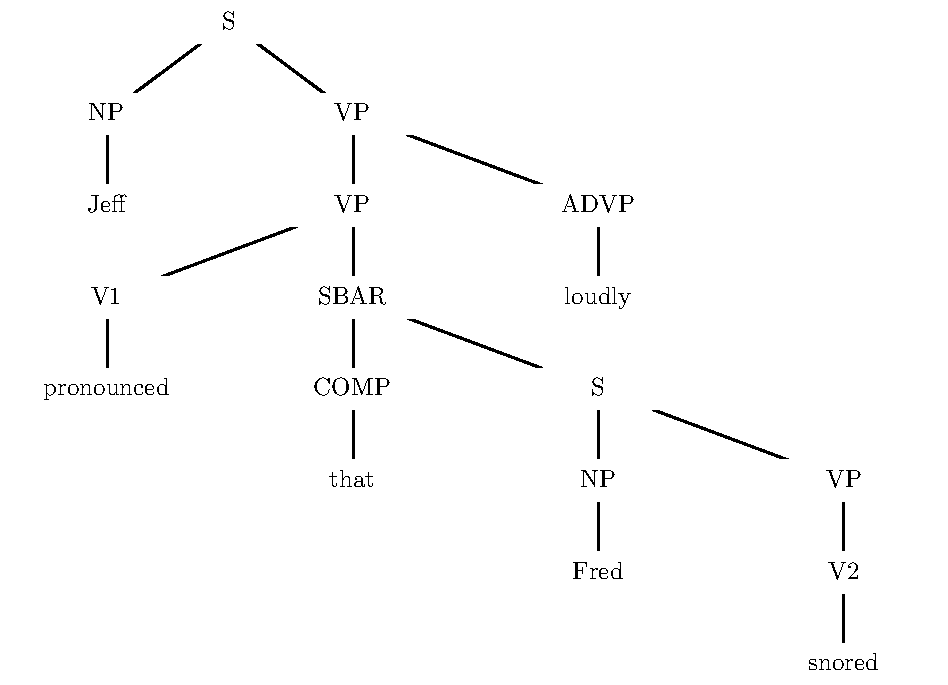
\includegraphics[]{h2-2-parsetree2.pdf}}
\caption{Parse Tree 2: Jeff saying loudly that Fred snored.}
\label{fig:parse_tree_2}
\end{figure}

\begin{align*}
P_{\tau_1} &= [ P(\n{S} \rightarrow \n{NP VP}) * P(\n{VP} \rightarrow \n{VP ADVP}) * P(\n{VP} \rightarrow \n{V1 SBAR}) * P(\n{SBAR} \rightarrow \n{COMP S}) \\
&* P(\n{S} \rightarrow \n{NP VP}) * P(\n{VP} \rightarrow \n{V2}) \\ 
&* P(\n{NP} \rightarrow \n{Jeff}) * P(\n{V1} \rightarrow \n{pronounced}) * P(\n{COMP} \rightarrow \n{that}) * P(\n{NP} \rightarrow \n{Fred}) \\
&* P(\n{V2} \rightarrow \n{snored}) * P(\n{ADVP} \rightarrow \n{loudly}) ] \\
&= \left[ 1 * \frac{1}{3} * 1 * 1 *\frac{1}{3} * \frac{1}{3} * \frac{1}{6} * \frac{1}{3} * 1 * \frac{1}{6} * \frac{1}{3} * \frac{1}{3} \right] \\
&= \frac{1}{26244}
\end{align*}

\subsection{Modifying Non-Terminals}

Modify rule $\n{VP} \rightarrow \n{VP ADVP}$ to $\n{VP} \rightarrow \n{V2 ADVP}$ such that it is impossible for ADVP to follow a verb phrase (and only follows single verbs, hence eliminating "high" attachments.)

This will allow the first parse tree in Figure \ref{fig:parse_tree_1} to retain its probability since the ADVP portion of the parse tree will simply be modified to $\n{VP} \rightarrow \n{V2 ADVP}$. However, the second parse tree in Figure \ref{fig:parse_tree_2} will have a probability of 0 since $\n{VP} \rightarrow \n{VP ADVP}$ does not exist anymore, hence the ADVP loudly cannot possibly refer to the entire VP "pronounced that Fred snored".

\section{CKY Algorithm}

Since the tree is balanced and since sentences are only of length $n=2^x$, then instead of searching over all $s$, we can just divide the sentence length into half each time. Hence, the algorithm can be

\begin{itemize}
\item \textbf{Base Case:} for all $i = 1 ... n$, for all $X \in N$
\[ \pi(i,i,X) = \begin{cases}
q(X \rightarrow x_i),& \n{if } X \rightarrow x_i \in R \\
0,& \n{otherwise}
\end{cases}
\]
\item \textbf{Recursive Case:}
\begin{itemize}
\item For all $X \in N$, calculate
\[ \pi(i, j, X) = \max_{X \rightarrow YZ \in R} \left[ q(\n{X} \rightarrow \n{Y Z}) * \pi\left(i, \frac{j}{2}, Y\right) * \pi\left(\frac{j}{2}+1, j, Z\right) \right] \]
\end{itemize}
\item \textbf{Return:} 
\[\pi(1, n, S) = \max_{t \in \tau_G(s)} p(t)\]
\end{itemize}

This speeds up the algorithm significantly, giving it a complexity of $O(\log{n} |N|^3)$ (please don't kill me if I get the complexity wrong).

\end{document}
